\section{Notation and Basic Concepts}\label{sec:notation}

\alex{Novelty here: Defining tensor networks on hypergraphs, to ease the relation with graphical models (avoid graph duality).}

We in this section introduce the tensor network formalism and the basic architecture. % and later show how the probabilistic and logical framework are covered.
First, the considered variables and tensors are explained.
Followed by the explanation of tensor calculations, mainly tensor products and contractions.
Finally, the main architecture, the \emph{\ComputationActivationNetwork{}}, is defined.

%\subsection{Categorical Variables and Representations}
%\label{sec:categorical-variables-and-representations}
%
%We will investigate systems, which are described by a set of properties, each called categorical variables.
%
%\begin{definition}
%    \label{def:atomic-factored-representation}
%    An \emph{atomic representation} of a system is described by a \emph{categorical variables} $\catvariable$ taking values $\catindex$ in a finite set
%    \[  [\catdim]\coloneqq \{0,\ldots, \catdim-1\} \]
%    of cardinality $\catdim$. The values $x\in[m]$ are called the \emph{states} of the variable. A \emph{factored representation} of a system is a set of categorical variables $\catvariableof{\atomenumerator}$, where $\atomenumeratorin$, taking values in $[\catdimof{\atomenumerator}]$.
%\end{definition}
%We abbreviate lists $\catvariables$ of categorical variables by $\shortcatvariables$.
%Furthermore, we will always notate categorical variables by large literals and indices by small literals, possible with other letters such as $\catvariable,\selvariable,\indvariable,\datvariable$ and corresponding values $\catindex,\selindex,\indindex,\datindex$.

\subsection{Tensors}
\label{sec:tensors}

Tensors are multiway arrays and a generalization of vectors and matrices to higher orders.
We will first provide a formal definition as real maps from index sets enumerating the coordinates of vectors, matrices and larger order tensors.

\begin{definition}[Tensor]
    \label{def:tensor}
    For $\atomenumeratorin$, let $\catdimof{\atomenumerator}\in\nn$ and let $\catvariableof{\atomenumerator}$ be categorical variables with values in $[\catdimof{\atomenumerator}]$.
    A tensor $\hypercoreat{\catvariables}$ of order $\catorder$ and with leg dimensions $\catdimof{0},\dots,\catdimof{\atomorder-1}$ is defined through its coordinates
    \begin{align*}
        \hypercoreat{\indexedcatvariableof{0},\ldots,\indexedcatvariableof{\catorder-1}} \in \rr
    \end{align*}
    for index tuples
    \begin{align*}
        \catindexof{0},\ldots,\catindexof{\catorder-1} \in \facstates \, .
    \end{align*}
    Tensors $\hypercoreat{\catvariables}$, also denoted by $\hypercoreat{\shortcatvariables}$, are elements of the tensor space
    \begin{align*}
        \bigotimes_{\atomenumeratorin} \rr^{\catdimof{\atomenumerator}} \,,
    \end{align*}
    which is a linear space, enriched with the operations of coordinate wise summation and scalar multiplication. We call a tensor $\hypercoreat{\shortcatvariables}$ boolean, when $\imageof{\hypercore}\subset[2]$, i.e. all coordinates are either $0$ or $1$.
\end{definition}

This notation of tensors opposed to its notation through ordered indices as common in tensor calculus, facilitates writing down contractions along individual legs and other operations.
Occasionally, when the categorical variables of a tensor are clear from the context, we will omit the notation of the variables. %further abbreviate $\hypercoreat{\catvariables}$ by $\hypercore$.

\begin{example}[Trivial Tensor]
    \label{exa:trivialTensor}
    The trivial tensor
    \begin{align*}
        \onesat{\shortcatvariables} \in \facspace
    \end{align*}
    is defined by all coordinates being $1$, that is for all $\catindices\in\facstates$
    \begin{align*}
        \onesat{\indexedshortcatvariables} = 1 \, .
    \end{align*}
\end{example}

We are now ready to provide the link between tensors and states of systems with factored representations.
To this end, we define the one-hot encoding of a state, which is a bijection between the states and the basis elements of a tensor space.

\begin{definition}[One-hot encodings to Atomic Representations]
    \label{def:onehotenc}
    Given an atomic system described by the categorical variable $\catvariable$, we define for each $\catindex\in[\catdim]$ the basis vector $\onehotmapofat{\catindex}{\catvariable}$ by the coordinates
    \begin{align}
        \onehotmapofat{\catindex}{\catvariable=\tilde{\catindex}}
        = \begin{cases}
              1 & \ifspace \catindex=\tilde{\catindex} \\
              0 & \text{else} \, .
        \end{cases}
    \end{align}
    The \emph{one-hot encoding of states} $\catindex\in[\catdim]$ of the atomic system described by the categorical variable $\catvariable$ is the map
    $ \onehotmap: [\catdim] \rightarrow \rr^\catdim $
    which maps $\catindex \in [\catdim]$ to the basis vectors $\onehotmapofat{\catindex}{\catvariable}$.
\end{definition}

The basis vectors $\onehotmapofat{\catindex}{\catvariable}$ are tensors of order $1$ and leg dimension $\catdim$ of the structure
\begin{align}
    \onehotmapofat{\catindex}{\catvariable}
    = \begin{bmatrix}
          0 & \cdots & 0 & 1 & 0 & \cdots & 0
    \end{bmatrix}^T \, ,
\end{align}
where the $1$ is at the $\catindex$-th coordinate of the vector.

\subsection{Contractions and Tensor Networks}
Contractions are the central manipulation operation on sets of tensors.
To introduce them, a graphical illustration of sets of tensors is explained, which we also call tensor networks.

\subsubsection{Graphical Illustration}

% Diagrammatic representation in factor graphs
We will use the standard visualization %by factor graphs as a diagrammatic illustration of sets 
of tensors, where they are represented by blocks with lines depicting the axes of the tensor blocks and each axis is assigned with a categorical variable $\catvariableof{\atomenumerator}$,  or sometimes their index or dimension. %, see \figref{fig:tensors}.

% \begin{figure}[h]
\begin{center}
    \begin{tikzpicture}[scale=0.35,thick] % , baseline = -3.5pt


\begin{scope}[shift={(-17,0)}]

\node[anchor=center] (text) at (-3,0) {$a)$};

\draw (-1,1) rectangle (10,-1);
\node[anchor=center] (text) at (4.5,0) {\corelabelsize $\hypercoreof{\edge}$};

\draw (0,-1)--(0,-3) node[midway,left] {\colorlabelsize $\catvariableof{0}$};
\draw (3,-1)--(3,-3) node[midway,left] {\colorlabelsize $\catvariableof{1}$};
\node[anchor=center] (text) at (3,-4) {$\cdots$};
\draw (9,-1)--(9,-3) node[midway,right] {\colorlabelsize $\catvariableof{\atomorder\shortminus1}$};

\node [circle, draw, thick, fill=\nodegrayscale, minimum size = \nodeminsize] (P1) at (0,-4) {\colorlabelsize $\catvariableof{0}$};
\node [circle, draw, thick, fill=\nodegrayscale, minimum size = \nodeminsize] (P2) at (3,-4) {\colorlabelsize $\catvariableof{1}$};
\node[anchor=center] (text) at (6,-4) {$\cdots$};

\node [circle, draw, thick, fill=\nodegrayscale, minimum size = \nodeminsize] (P3) at (9,-4) {};

\node[anchor=center] (text) at (9,-4) {\colorlabelsize $\catvariableof{\atomorder-1}$};


\end{scope}


\node[anchor=center] (text) at (-2,0) {$b)$};

\node [circle, draw, thick, fill=\nodegrayscale, minimum size = \nodeminsize] (P1) at (0,-3) {\colorlabelsize $\catvariableof{0}$};
\node [circle, draw, thick, fill=\nodegrayscale, minimum size = \nodeminsize] (P2) at (3,-3) {\colorlabelsize $\catvariableof{1}$};

\node[anchor=center] (text) at (6,-3) {$\cdots$};

\node [circle, draw, thick, fill=\nodegrayscale, minimum size = \nodeminsize] (P3) at (9,-3) {};

\node[anchor=center] (text) at (9,-3) {\colorlabelsize $\catvariableof{\atomorder-1}$};


\draw (P1) to[bend right=-25] (4.5,0);
\draw (P2) to[bend right=-10] (4.5,0);
\draw (P3) to[bend right=25] (4.5,0);
\node[anchor=center] (text) at (4.5,0.5) {$\edge$};


\begin{scope}[shift={(16,2)}]

\node[anchor=center] (text) at (-3,-2) {$c)$};

\draw (-1,-1) rectangle (5,-3);
\node[anchor=center] (text) at (2,-2) {\corelabelsize $\hypercoreof{\edge}$};
\draw (0,-3)--(0,-5) node[midway,left] {\colorlabelsize $\catvariableof{0}$};
\draw (1.5,-3)--(1.5,-5) node[midway,left] {\colorlabelsize $\catvariableof{1}$};
\node[anchor=center] (text) at (3,-4) {$\cdots$};
\draw (4,-3)--(4,-5) node[midway,right] {\colorlabelsize $\catvariableof{\atomorder\shortminus1}$};

\end{scope}

%\drawatomcore{3.5}{-8}{$\probtensor$}
%\drawatomindices{3.5}{-12}	
%\draw (5.5,-9)--(5.5,-7) node[midway,right] {\colorlabelsize $\catvariableof{\exformula}$};

\end{tikzpicture}
\end{center}
% 	\caption{Depiction of Tensors: Highlighting the tensor by a blockwise notation with axes denoted by open legs represented by the variables $\catvariableof{\atomenumerator}$.
% 	}\label{fig:tensors}
% \end{figure}

This depiction scheme has been established in the literature as wiring diagrams (see \cite{landsberg_tensors_2011} and dates back at least to the work \cite{penrose_spinors_1987}.
Along this line, we represent vectors %and their generalization to tensors 
by blocks with one leg. % representing its indices.
The basis vectors being one-hot encodings of states are in this scheme represented by
\begin{center}
    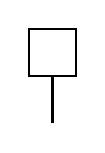
\begin{tikzpicture}[scale=0.3,thick] % , baseline = -3.5pt

\draw (1,1) rectangle (3,3);
\node[anchor=center] (text) at (2,2) {\corelabelsize $\onehotmapof{\catindex}$};
\draw (2,-1)--(2,1) node[midway,right] {\colorlabelsize $\catvariable$};

\end{tikzpicture}
\end{center}
%where $\tilde{\catindex}$ is an indexed represented by an open leg.
Assigning $\catindex$ to the categorial variable $X$ will retrieve the $\catindex$th coordinate (with value $1$), whereas all other assignments will retrieve the coordinate values $0$.
Drawing on the interpretation of tensors by hyperedges we can continue with the definition of tensor networks.
\begin{definition}[Tensor Network]
    \label{def:tensorNetwork}
    Let $\graph=(\nodes,\edges)$ be a hypergraph with nodes decorated by categorical variables $\catvariableof{\node}$ with dimensions
    $ \catdimof{\node} \in \nn $
    and hyperedges $\edge\in\edges$ decorated by core tensors
    \[ \hypercoreofat{\edge}{\catvariableof{\edge}} \in \bigotimes_{\node\in\edge}\rr^{\catdimof{\node}} \, , \]
    where we denote by $\catvariableof{\edge}$ the set of categorical variables $\catvariableof{\node}$ with $\node\in\edge$.
    Then we call the set
    \[ \tnetofat{\graph}{\catvariableof{\nodes}} = \{\hypercoreofat{\edge}{\catvariableof{\edge}}  \wcols \edge\in\edges\} \]
    the Tensor Network of the decorated hypergraph $\graph$.
    The set of tensor networks on $\graph$, such that all tensors have non-negative coordinates, is denoted by $\tnsetof{\graph}$.
\end{definition}

As examples we now present the $\cpformat$ and the $\ttformat$ formats in our hypergraph notation.

\begin{example}[The $\cpformat$ format]
    The Candecomp-Parafac ($\cpformat$ (\cite{hitchcock_expression_1927}) tensor format corresponds in our notation with a hypergraph (see \figref{fig:CPHypergraph})
    \begin{itemize}
        \item Nodes by $\catvariableof{[\catorder]}$ and a single hidden variable $\decvariable$, decorated by dimensions $\catdimof{[\catorder]}$ and $\decdim$.
        \item Edges by
        \begin{align*}
            \left\{\edgeof{\catenumerator}=(\catvariableof{\catenumerator},\decvariable) \wcols \catenumeratorin \right\}
        \end{align*}
        each decorated by a matrix $\hypercoreofat{\edgeof{\catenumerator}}{\catvariableof{\catenumerator},\decvariable}$.
    \end{itemize}

    \begin{figure}
        \begin{center}
            \input{../tikz_pics/notation_basic_concepts/cp_hypergraph.tex}
        \end{center}
        \caption{Hypergraph to a $\cpformat$ format.
        a) Node-centric design.
        b) Corresponding tensor-network on the edges of the hypergraph.}\label{fig:CPHypergraph}
    \end{figure}

\end{example}

\begin{example}[The $\ttformat$ format]\label{exa:ttFormat}
    The Tensor-Train ($\ttformat$) format (see \cite{oseledets_tensor-train_2011}) corresponds in our notation to a hypergraph (see \figref{fig:TTHypergraph}) defined by
    \begin{itemize}
        \item nodes $\catvariableof{[\catorder]}$ and hidden variables $\decvariableof{[\catorder-1]}$, each decorated by a dimension $\catdimof{[\catorder]}$ and $\decdimof{[\catorder-1]}$,
        \item edges
        \begin{align*}
            \big\{\edgeof{0}=\{\catvariableof{0},\decvariableof{0}\}\big\} \cup
            \big\{\edgeof{\catenumerator}=\{\decvariableof{\catenumerator-1},\catvariableof{\catenumerator},\decvariableof{\catenumerator}\} \wcols \catenumerator\in\{1,\ldots,\catorder-2\}\big\} \cup
            \big\{\edgeof{\catorder-1}=\{\decvariableof{\catorder-2},\catvariableof{\catorder-1}\}\big\}
        \end{align*}
        each decorated by a tensor of order 3 (respectively 2 for $\catenumerator\in\{0,\seldim-1\}$).
    \end{itemize}
    \begin{figure}
        \begin{center}
            \begin{tikzpicture}[scale=0.35,thick]

                \begin{scope}[shift={(-22,-2)}]
                    \coordinate[label=left:$a)$] (A) at (-2,4);

                    \node[circle, draw, thick, fill=\nodegrayscale, minimum size = \nodeminsize] (A) at (0,0) {};
                    \node[anchor=center] (A) at (0,0) {\corelabelsize $\catvariableof{0}$};
                    \node[circle, draw, thick, fill=\nodegrayscale, minimum size = \nodeminsize] (A) at (4,0) {};
                    \node[anchor=center] (A) at (4,0) {\corelabelsize $\catvariableof{1}$};


                    \coordinate[label=below:$\hdots $] (A) at (10.5,4);
                    \coordinate[label=below:$\hdots $] (A) at (10.5,0);

                    \node[circle, draw, thick, fill=\nodegrayscale, minimum size = \nodeminsize] (A) at (2,4) {};
                    \node[anchor=center] (A) at (2,4) {\corelabelsize $\decvariableof{0}$};
                    \node[circle, draw, thick, fill=\nodegrayscale, minimum size = \nodeminsize] (A) at (6,4) {};
                    \node[anchor=center] (A) at (6,4) {\corelabelsize $\decvariableof{1}$};

                    %\coordinate[label=above:$e_0$] (A) at (0.5,1.6);
                    %\node[anchor=south] (A) at (0.5,1.6) {\colorlabelsize $e_0$};
                    \draw (0.5,1) -- (1.5,3) node[midway,left] {\colorlabelsize $e_0$};
%                    \draw (2,2)  to[bend right=30] (0.5,1);
%                    \draw (2,2)  to[bend left=30] (3.5,1);
%                    \draw (2,2) -- (2,2.9);

                    \node[anchor=south] (A) at (4,2) {\colorlabelsize $e_1$};
                    \draw (4,2)  to[bend right=-30] (2.5,3);
                    \draw (4,2)  to[bend left=-30] (5.5,3);
                    \draw (4,2) -- (4,1.1);

                    \node[anchor=south] (A) at (8,2) {\colorlabelsize $e_2$};
                    \draw (8,2)  to[bend right=-30] (6.5,3);
                    \draw (8,2)  to[bend left=-30] (9.5,3);
                    \draw (8,2) -- (8,1.1);

                    \begin{scope}[shift={(3,0)}]

                        \node[anchor=south] (A) at (10,2) {\colorlabelsize $e_{\catorder-2}$};
                        \draw (10,2)  to[bend right=-30] (8.5,3);
                        \draw (10,2)  to[bend left=-30] (11.5,3);
                        \draw (10,2) -- (10,1.1);

                        %\node[anchor=south] (A) at (0.5,1.6) {\colorlabelsize $e_0$};
                        \draw (13.5,1) -- (12.5,3) node[midway,right] {\colorlabelsize $e_{\catorder-1}$};

                        %\coordinate[label=above:$e_{\catorder-1}$] (A) at (11,1.6);
                        %\draw (12,2)  to[bend right=30] (10.5,1);
                        %\draw (12,2)  to[bend left=30] (13.5,1);
                        %\draw (12,2) -- (12,2.9);

                        \node[circle, draw, thick, fill=\nodegrayscale, minimum size = \nodeminsize] (A) at (12,4) {};
                        \node[anchor=center] (text) at (12,4) {\corelabelsize $\decvariableof{\catorder\shortminus2}$};

                        \node[circle, draw, thick, fill=\nodegrayscale, minimum size = \nodeminsize] (A) at (14,0) {};
                        \node[] (text) at (14,0) {\corelabelsize $\catvariableof{\catorder\shortminus1}$};
                    \end{scope}
                \end{scope}

                \coordinate[label=left:$b)$] (A) at (-2,2);

                \draw (-1,-1) rectangle (1,1);
                \node[anchor=center] (A) at (0,0) {\corelabelsize $\hypercoreof{0}$};
                \draw (0,-1)--(0,-2.5) node[midway,right] {\colorlabelsize $\catvariableof{0}$};

                \draw (1,0) -- (3,0) node[midway,above] {\colorlabelsize $\decvariableof{0}$};

                \draw (3,-1) rectangle (5,1);
                \node[anchor=center] (A) at (4,0) {\corelabelsize $\hypercoreof{1}$};
                \draw (4,-1)--(4,-2.5) node[midway,right] {\colorlabelsize $\catvariableof{1}$};

                \draw (5,0) -- (6.5,0) node[midway,above] {\colorlabelsize $\decvariableof{1}$};

%    \coordinate[label=below:$\hdots $] (A) at (9,0.35);
                \node[anchor=center] (text) at (8,0) {$\hdots$};

                \draw (9.5,0) -- (11,0) node[midway,above] {\colorlabelsize $\decvariableof{\catorder\shortminus2}$};;
                \draw (11,-1) rectangle (13,1);
                \node[anchor=center] (A) at (12,0) {\corelabelsize $\hypercoreof{\catorder\shortminus1}$};
                \draw (12,-1)--(12,-2.5) node[midway,right] {\colorlabelsize $\catvariableof{\catorder\shortminus1}$};


            \end{tikzpicture}
        \end{center}
        \caption{Hypergraph to a $\ttformat$ format.
        a) Node-centric design.
        b) Corresponding tensor-network on the edges of the hypergraph.}\label{fig:TTHypergraph}
    \end{figure}

\end{example}

\subsubsection{Tensor Product}
Let us now exploit the developed graphical representations to define contractions of tensor networks.
The simplest contraction is the tensor product, which maps a pair of two tensors with distinct variables onto a third tensor and has an interpretation by coordinate wise products.
Such a contraction corresponds with a tensor network of two tensors with disjoint variables.

\begin{definition}[Tensor Product]
    \label{def:tensorProduct}
    Let there be two tensors
    \begin{align*}
        \hypercoreat{\shortcatvariables} \in \facspace  \andspace \sechypercoreat{\secshortcatvariables} \in \secfacspace
    \end{align*}
    with different categorical variables assigned to its axes.
    Then their tensor product is the map
    \begin{align*}
        \contractionof{\hypercoreat{\shortcatvariables},\sechypercoreat{\secshortcatvariables}}{\shortcatvariables,\secshortcatvariables}
        \in \left(\facspace\right) \otimes \left(\secfacspace \right)
        %:  \left(\facstates\right) \times \left(\secfacstates\right) \rightarrow \rr
    \end{align*}
    defined coordinatewise for tuples of $\catindices\in\facstates$ and $\seccatindices\in\secfacstates$ as
    \begin{align*}
        & \contractionof{\hypercoreat{\shortcatvariables},\sechypercoreat{\secshortcatvariables}}{\indexedcatvariables,\indexedseccatvariables} \\
        &\quad\quad :=  \hypercoreat{\indexedcatvariables}\cdot \sechypercoreat{\indexedseccatvariables} \, .
    \end{align*}
\end{definition}

%\janina{The subsection title also says contraction. After defining contraction, we could also define normalization and conditional probability tensors. This should be here, since the arrows are needed in the next subsections.}

\subsection{Generic Contractions}


Contractions of Tensor Networks $\extnet$ are operations to retrieve single tensors by summing products of tensors in a network over common indices.
We will define contractions formally by specifying just the indices not to be summed over.

When some of the variables are not appearing as leg variables, we define the contraction as being a tensor product with the trivial tensor $\ones$ carrying the legs of the missing variables.

\begin{definition}
    \label{def:contraction}
    Let $\tnetof{\graph}$ be a tensor network on a decorated hypergraph $\graph=(\nodes,\edges)$.
    For any subset $\secnodes\subset\nodes$ we define the contraction to be the tensor (for an example see \figref{fig:contraction})
    \begin{align}
        \contractionof{\tnetof{\graph}}{\secnodevariables} \in \bigotimes_{\node\in\secnodes} \rr^{\catdimof{\node}}
    \end{align}
    defined coordinatewise by the sum
    \begin{align}
        \contractionof{\tnetof{\graph}}{\indexedcatvariableof{\secnodes}} =
        \sum_{\catindexof{\nodes/\secnodes} \in\,\nodestatesof{\nodes/\secnodes}}
        \left( \prod_{\edge\in\edges}\hypercoreofat{\edge}{\indexedcatvariableof{\edge}} \right) \, .
    \end{align}
    We call $\secnodevariables$ the open variables of the contraction.
\end{definition}

To ease notation, we will often omit the set notation by brackets $\{\cdot\}$ and specify the tensors to be contracted with the delimiter "," (see e.g. \exaref{exa:matrixProduct}).

\begin{figure}
    \begin{center}
        \begin{tikzpicture}[scale=0.35,thick]

    \draw (-5,-1) rectangle (9,-3);
    \node[anchor=center] (text) at (2,-2) {\corelabelsize $\contractionof{\hypercoreof{\edge_0},\hypercoreof{\edge_1},\hypercoreof{\edge_2}}{\catvariableof{1},\catvariableof{3}}$};
    \draw (0,-3)--(0,-5) node[midway,left] {\colorlabelsize $\catvariableof{1}$};
    \draw (4,-3)--(4,-5) node[midway,left] {\colorlabelsize $\catvariableof{3}$};

    \node[anchor=center] (text) at (11.5,-2) {${=}$};

    \begin{scope}
        [shift={(15,0)}]

        \draw (-1,-1) rectangle (5,-3);
        \node[anchor=center] (text) at (2,-2) {\corelabelsize $\hypercoreof{\edge_0}$};
        \draw (0,-3)--(0,-4) node[midway,right] {\colorlabelsize $\catvariableof{0}$};
        \draw (-1,-4) rectangle (1,-6);
        \node[anchor=center] (text) at (0,-5) {\corelabelsize $\ones$};

        \draw (2,-3)--(2,-5) node[midway,right] {\colorlabelsize $\catvariableof{1}$};
        \draw (4,-3)--(4,-5) node[midway,right] {\colorlabelsize $\catvariableof{2}$};


        \draw (6,-1) rectangle (10,-3);
        \node[anchor=center] (text) at (8,-2) {\corelabelsize $\hypercoreof{\edge_2}$};
        \draw (7,-3)--(7,-5) node[midway,right] {\colorlabelsize $\catvariableof{2}$};
        \draw (9,-3)--(9,-5) node[midway,right] {\colorlabelsize $\catvariableof{3}$};


        \draw (1,-7) rectangle (5,-9);
        \node[anchor=center] (text) at (3,-8) {\corelabelsize $\hypercoreof{\edge_1}$};
        \draw (2,-5)--(2,-7); % node[midway,left] {\colorlabelsize $\catvariableof{1}$};
        \draw (4,-5) to[bend right=20]  (7,-6); % node[midway,left] {\colorlabelsize $\catvariableof{2}$};
        \draw (4,-7) to[bend right=-20]  (7,-6);

        \draw[fill] (2,-6) circle (\dotsize);
        \draw (2,-6) to[bend right=20] (-1,-8); % node[midway, right]{\colorlabelsize $\catvariableof{1}$};
        \node[anchor=center] (text) at (-2,-8) {\colorlabelsize $\catvariableof{1}$};

        \draw[fill] (7,-6) circle (\dotsize);
        \draw (7,-5) -- (7,-6);
        \draw (7,-6)--(7,-7) node[midway,right] {\colorlabelsize $\catvariableof{2}$};

        \draw (6,-7) rectangle (8,-9);
        \node[anchor=center] (text) at (7,-8) {\corelabelsize $\ones$};

    \end{scope}


\end{tikzpicture}
    \end{center}
    \caption{
        Graphical depiction of a tensor network contraction with the open variables $\catvariableof{1},\catvariableof{3}$.
    }\label{fig:contraction}
\end{figure}

%We explain normalization of tensors along specific legs here by an example and define it properly in~\ref{}.
%This normalization corresponds to conditional probabilities, if the considered tensor $\hypercore$ describes an unnormalized probability distribution over its states.
%For a tensor $\hypercoreat{X_{[2]}} \in \mathbb{R}^{m_0}\otimes\mathbb{R}^{m_1}$ and any $\secexrandindin$ we depict the slice $\hypercoreat{\catvariableof{0}|X_1=x_1}\in\mathbb{R}^{m_0}$ and $\hypercoreat{\catvariableof{0}|X_1}\in\mathbb{R}^{m_0}\otimes\mathbb{R}^{m_1}$ defined by a normalization operation as
%\begin{center}
%    \begin{tikzpicture}[scale=0.3, thick] % , baseline = -3.5pt

\draw (-21,-1) rectangle (-15,-3);
\node[anchor=center] (text) at (-18,-2) {\small $\condprobof{\exrandom}{\secexrandom}$};
\draw[->]  (-20,-3)--(-20,-5) node[midway,left] {\tiny $\exrandom$}; 

\draw[<-]  (-16,-3)--(-16,-5) node[midway,left] {\tiny $\secexrandom$}; 
\draw[dashed] (-15,-5) rectangle (-17,-7); 
\node[anchor=center] (text) at (-16,-6) {\small $\onehotmapof{\catindexof{\secexrandom}}$};

\node[anchor=center] (text) at (-13,-2) {${=}$};


\begin{scope}[shift={(0,6)}]

\draw (-11,-1) rectangle (-5,-3);
\node[anchor=center] (text) at (-8,-2) {\small $\probof{\exrandom,\secexrandom}$};
\draw[->]  (-10,-3)--(-10,-5) node[midway,left] {\tiny $\exrandom$}; 
\draw[->]  (-6,-3)--(-6,-5) node[midway,left] {\tiny $\secexrandom$};
\draw[dashed] (-7,-5) rectangle (-5,-7); 
\node[anchor=center] (text) at (-6,-6) {\small $\onehotmapof{\catindexof{\secexrandom}}$};

\end{scope}

\draw (-12,-2) -- (-4,-2);

\begin{scope}[shift={(0,-2)}]

\draw (-11,-1) rectangle (-5,-3);
\node[anchor=center] (text) at (-8,-2) {\small $\probof{\exrandom,\secexrandom}$};
\draw[->]  (-10,-3)--(-10,-5) node[midway,left] {\tiny $\exrandom$}; 
\draw (-11,-5) rectangle (-9,-7); 
\node[anchor=center] (text) at (-10,-6) {$\ones$};
\draw[->]  (-6,-3)--(-6,-5) node[midway,left] {\tiny $\secexrandom$};
\draw[dashed] (-7,-5) rectangle (-5,-7); 
\node[anchor=center] (text) at (-6,-6) {\small $\onehotmapof{\catindexof{\secexrandom}}$};

\end{scope}

\end{tikzpicture}
%\end{center}
%This way any entrywise positive tensor can be normalized to form a probability distribution by conditioning on the empty set $\emptyset$.

\subsection{Normalizations}

%% Directionality by Normalization
\begin{definition}
    \label{def:normalization}
    The normalization of a tensor $\hypercorewithnodes$ on incoming nodes $\innodes\subset\nodes$ and outgoing nodes $\outnodes\subset\nodes/\innodes$ is the tensor $\normalizationofwrt{\hypercorewithnodes}{\catvariableof{\outnodes}}{\catvariableof{\innodes}}$ defined for $\catindexof{\innodes}$ as
    \begin{align*}
        \normalizationofwrt{\hypercorewithnodes}{\catvariableof{\outnodes}}{\indexedcatvariableof{\innodes}}
        = \begin{cases}
              \frac{\contractionof{\hypercore}{\catvariableof{\outnodes},\indexedcatvariableof{\innodes}}}{\contractionof{\hypercore}{\indexedcatvariableof{\innodes}}} & \ifspace \contractionof{\hypercore}{\indexedcatvariableof{\innodes}} \neq 0 \\
              \frac{1}{\prod_{\node\in\outnodes}\catdimof{\node}}\onesat{\catvariableof{\outnodes}} & \text{else}
        \end{cases} \, .
    \end{align*}
    We say that $\hypercorewithnodes$ is normalized with incoming nodes $\incomingnodes\subset\nodes$, if
    \begin{align*}
        \hypercorewithnodes
        = \normalizationofwrt{\hypercorewithnodes}{\catvariableof{\nodes/\innodes}}{\catvariableof{\innodes}} \, .
    \end{align*}
\end{definition}

Directionality thus represents constraints on the structure of tensors, namely that the sum over outgoing trivializes the tensor.
%% Diagrammatic notation
In our graphical tensor notation, we depict normalized tensors by directed hyperedges (a), which are decorated by directed tensors (b), for example:
\begin{center}
    \begin{tikzpicture}[scale=0.35,thick] % , baseline = -3.5pt

    \node[anchor=center] (text) at (-2,0) {$a)$};

    \node [circle, draw, thick, fill=\nodegrayscale, minimum size = \nodeminsize] (P1) at (0,-3) {\colorlabelsize $\catvariableof{0}$};
    \node [circle, draw, thick, fill=\nodegrayscale, minimum size = \nodeminsize] (P2) at (3,-3) {\colorlabelsize $\catvariableof{1}$};

%\node[anchor=center] (text) at (6,-3) {$\cdots$};
    \node [circle, draw, thick, fill=\nodegrayscale, minimum size = \nodeminsize] (P3) at (6,-3)  {\colorlabelsize $\catvariableof{2}$};

    \node [circle, draw, thick, fill=\nodegrayscale, minimum size = \nodeminsize] (P4) at (9,-3)  {\colorlabelsize $\catvariableof{3}$};

    \node[anchor=center] (text) at (9,-3) {\colorlabelsize $\catvariableof{3}$};


    \draw[midarrow]
    (4.5,0) to[bend right=25] (P1);
    \draw[midarrow]
    (4.5,0) to[bend right=10] (P2);
    \draw[midarrow]
    (P3) to[bend right=10] (4.5,0);
    \draw[midarrow]
    (P4) to[bend right=25] (4.5,0);

    \node[anchor=center] (text) at (4.5,0.5) {$\edge$};


    \begin{scope}[shift={(20,0)}]

        \node[anchor=center] (text) at (-2,0) {$b)$};

        \draw (-1,-1) rectangle (7,-3);
        \node[anchor=center] (text) at (3,-2) {\corelabelsize $\hypercoreofat{\edge}{\catvariableof{0},\catvariableof{1},\catvariableof{2},\catvariableof{3}}$};
%\draw[->-] (0,-3)--(0,-5) node[midway,left] {\colorlabelsize $\catvariableof{0}$};
%\draw[->-] (1.5,-3)--(1.5,-5) node[midway,left] {\colorlabelsize $\catvariableof{1}$};
%\node[anchor=center] (text) at (3,-4) {$\cdots$};
%\draw[->-] (4,-3)--(4,-5) node[midway,right] {\colorlabelsize $\catvariableof{\atomorder-1}$};


        \draw[midarrow]  (0,-3) -- (0,-5) node[midway,left] {\colorlabelsize $\catvariableof{0}$};
        \draw[midarrow]
        (2,-3)--(2,-5) node[midway,left] {\colorlabelsize $\catvariableof{1}$};
        \draw[midarrow]
        (4,-5)--(4,-3) node[midway,left] {\colorlabelsize $\catvariableof{2}$};
        \draw[midarrow]
        (6,-5)--(6,-3) node[midway,right] {\colorlabelsize $\catvariableof{3}$};
    \end{scope}


\end{tikzpicture}
\end{center}

\subsection{Function encoding and \ComputationActivationNetworks{}}

\alex{Might need to discuss image enumerating maps!}

Let us now encode functions between the state sets of systems in factored representation.

\begin{definition}[Basis encoding of maps between state sets]
    \label{def:functionRepresentation}
    Let there be two systems with factored representations by variables $\shortcatvariables$ and $\headvariables$, and a map
    \begin{align*}
        \statesetfunction\defcols\facstates \rightarrow  \headstates
    \end{align*}
    between these state sets.
    Then the basis encoding of $\statesetfunction$ is a tensor
    \begin{align*}
        \bencodingofat{\statesetfunction}{\headvariables,\shortcatvariables}
        \in \left(\secfacspace\right) \otimes \left(\facspace\right)
    \end{align*}
    defined by
    \begin{align*}
        & \bencodingofat{\statesetfunction}{\headvariables,\shortcatvariables}
        \quad = \sum_{\catindices\in\facstates}
        \onehotmapofat{\statesetfunctionev{\shortcatindices}}{\headvariables} \otimes  \onehotmapofat{\shortcatindices}{\shortcatvariables} \, .
    \end{align*}
\end{definition}
Basis encodings are normalized tensors and are thus depicted as decorations of directed edges in hypergraphs:
\begin{center}
    \begin{tikzpicture}[scale=0.35,thick] % , baseline = -3.5pt


    \draw[->-] (0,-1)--(0,1) node[midway,left] {\colorlabelsize $\headvariableof{0}$};
    \draw[->-] (1.5,-1)--(1.5,1) node[midway,left] {\colorlabelsize $\headvariableof{1}$};
    \node[anchor=center] (text) at (3,-4) {$\cdots$};
    \draw[->-] (4,-1)--(4,1) node[midway,right] {\colorlabelsize $\headvariableof{\seccatorder\shortminus1}$};

    \draw (-1,-1) rectangle (5,-3);
    \node[anchor=center] (text) at (2,-2) {\corelabelsize $\bencodingof{\statesetfunction}$};
    \draw[-<-] (0,-3)--(0,-5) node[midway,left] {\colorlabelsize $\catvariableof{0}$};
    \draw[-<-] (1.5,-3)--(1.5,-5) node[midway,left] {\colorlabelsize $\catvariableof{1}$};
    \node[anchor=center] (text) at (3,-4) {$\cdots$};
    \draw[-<-] (4,-3)--(4,-5) node[midway,right] {\colorlabelsize $\catvariableof{\atomorder\shortminus1}$};


%\drawatomcore{3.5}{-8}{$\probtensor$}
%\drawatomindices{3.5}{-12}	
%\draw (5.5,-9)--(5.5,-7) node[midway,right] {\colorlabelsize $\catvariableof{\exformula}$};

\end{tikzpicture}
\end{center}

The entries of the basis encoding are defined by
\begin{align*}
    \bencodingofat{\statesetfunction}{\headvariables=\headindexof{[\seldim]},\indexedshortcatvariables}
    = \begin{cases}
          1 & \ifspace \statesetfunctionev{\shortcatindices}=\shortheadindices \\
          0 & \text{else}
    \end{cases}
\end{align*}

Based on these concepts the main architecture can be defined.

\begin{definition}[\ComputationActivationNetwork{} (\CompActNets{})]
    \label{def:realizableStatDistributions}
    Given a function $\sstat : \facstates \rightarrow \parspace$, and a hypergraph $\graph=(\nodes,\edges)$ with nodes $[\seldim]\subset\nodes$ containing the image coordinates of $\sstat$, we define the by $\sstat$ computable and by $\graph$ activated family of distributions by
    \begin{align*}
        \realizabledistsof{\sstat,\graph}
        = \left\{ \normalizationof{\bencodingofat{\sstat}{\headvariables,\shortcatvariables},\contractionof{\acttensor}{\headvariables} %\} \cup \{\hypercoreofat{\edge}{\sstatcatof{\edge}} \wcols \edgein \}
        }{\shortcatvariables}
              \wcols \acttensorat{\headvariableof{\nodes}} \in \tnsetof{\graph} \right\} \, .
    \end{align*}
    We refer to any member $\probat{\shortcatvariables}\in\realizabledistsof{\sstat,\graph}$ as a \ComputationActivationNetwork{}.
\end{definition}
To represent a \ComputationActivationNetwork{} two tensor networks are needed: $\beta^{\mathcal S}$ to represent the basis encoding of the sufficient statistic (also called \emph{computation network}) and $\xi$ to represent the tensor to contract with (also called \emph{activation network}).

% We write \(G_{EL}=([p],\{\{\ell\}:\ell\in[p]\})\) for the hypergraph of singleton edges and call it elementary activation graph. 
% An activation tensor on \(G_{EL}\) factorizes into a product of unary cores over \(Y_0,\dots,Y_{p-1}\).